En este capítulo se describe la construcción de la aplicación. Primero se expondrán las especificaciones de requisitos tanto externos, como funcionales. Después en el siguiente apartado se explicarán los diagramas UML del código, junto con explicaciones de todo el flujo del programa.\\

\section {Especificaci\'on de requisitos}

En esta sección se exponen todos los requisitos de la aplicación.\\

\subsection {Interfaces externos}

En esta sección se indican los requisitos externos a la aplicación.\\ \\
\textbf{Interfaces de usuario:}
\begin{itemize}
\item La interfaz de uso proporciona todo lo necesario para controlar la aplicación en su totalidad.\\
\end{itemize}
\textbf{Interfaces de hardware:}
\begin{itemize}
\item Se debe disponer de un dispositivo móvil y un ordenador.\\
\end{itemize}
\textbf{Interfaces de software:}
\begin{itemize}
\item La versión de Android del dispositivo móvil debe ser la 4.0 o superior.
\item El en la máquina remota se debe disponer de una aplicación VNC de tipo servidor.\\
\end{itemize}
\textbf{Interfaces de comunicación:}
\begin{itemize}
\item Tanto el cliente como el servidor deben disponer de una conexión a internet o estar ambos en la misma red local.\\
\end{itemize}
\subsection {Funciones}

Los siguientes requisitos funcionales definen las acciones que deben tener lugar en el software, aceptando, procesando las entradas y procesando, generando las salidas.\\

\textbf{Crear conexión:}
\begin{itemize}
\item Prioridad: Alta.
\item Estabilidad: Alta.
\item Descripción: Crea una nueva conexión y la añade a la lista de conexiones.
\item Entrada: Nombre de la conexión, IP, puerto, contraseña y calidad de imagen.
\item Salida: La conexión se añade a la lista.
\item Origen: Usuario.
\item Destino: Aplicación.
\item Necesita:
\item Acción: Crea una nueva conexión.
\item Precondición:
\item Postcondición: La conexión se añade a la lista de conexiones.
\item Efectos laterales: N/A.\\

\end{itemize}

\textbf{Editar conexión:}
\begin{itemize}
\item Prioridad: Alta.
\item Estabilidad: Alta.
\item Descripción: Se editan los datos de una determinada conexión.
\item Entrada: Nombre de la conexión, IP, puerto, contraseña y calidad de imagen.
\item Salida: La conexión con los datos modificados.
\item Origen: Usuario.
\item Destino: Aplicación.
\item Necesita:
\item Acción: Edita los datos de una conexión.
\item Precondición:
\item Postcondición: Los datos de la conexión se modifican.
\item Efectos laterales: N/A.\\

\end{itemize}

\textbf{Borrar conexión:}
\begin{itemize}
\item Prioridad: Alta.
\item Estabilidad: Alta.
\item Descripción: Se elimina una conexión.
\item Entrada:
\item Salida: La conexión se elimina de la aplicación.
\item Origen: Usuario.
\item Destino: Aplicación.
\item Necesita:
\item Acción: Elimina una conexión.
\item Precondición:
\item Postcondición: La conexión se borra de la aplicación.
\item Efectos laterales: Si la conexión esta en favoritos se borrará también ahí.\\

\end{itemize}

\textbf{Ver información de la conexión:}
\begin{itemize}
\item Prioridad: Alta.
\item Estabilidad: Alta.
\item Descripción: Muestra la información de una conexión.
\item Entrada:
\item Salida: Los datos de la conexión.
\item Origen: Usuario.
\item Destino: Usuario.
\item Necesita:
\item Acción: Muestra los datos de una conexión.
\item Precondición:
\item Postcondición: Se muestran los datos de una conexión.
\item Efectos laterales: N/A.\\

\end{itemize}

\textbf{Añadir conexión a favoritos:}
\begin{itemize}
\item Prioridad: Alta.
\item Estabilidad: Alta.
\item Descripción: Añade una conexión a la lista de favoritos del usuario.
\item Entrada: La conexión.
\item Salida: La conexión se añade a la lista de favoritos.
\item Origen: Usuario.
\item Destino: Aplicación.
\item Necesita: Acceso a la base de datos.
\item Acción: Añade la conexión a la lista de favoritos.
\item Precondición:
\item Postcondición: La conexión se añade a favoritos.
\item Efectos laterales: N/A.\\

\end{itemize}

\textbf{Borrar conexión de favoritos:}
\begin{itemize}
\item Prioridad: Alta.
\item Estabilidad: Alta.
\item Descripción: Borra una conexión de la lista de favoritos.
\item Entrada:
\item Salida: La conexión se elimina de favoritos.
\item Origen: Usuario.
\item Destino: Aplicación.
\item Necesita: Acceso a la base de datos.
\item Acción: Elimina una conexión de la lista de favoritos.
\item Precondición:
\item Postcondición: La conexión se borra de favoritos.
\item Efectos laterales: N/A.\\

\end{itemize}

\textbf{Ver lista de conexiones:}
\begin{itemize}
\item Prioridad: Alta.
\item Estabilidad: Alta.
\item Descripción: Se muestran todas las conexiones recientes.
\item Entrada:
\item Salida: La lista de conexiones recientes.
\item Origen: Usuario.
\item Destino: Usuario.
\item Necesita:
\item Acción: Se muestran las conexiones recientes.
\item Precondición: Tiene que existir al menos una conexión reciente.
\item Postcondición: Se muestra la lista de conexiones recientes.
\item Efectos laterales: N/A.\\

\end{itemize}

\textbf{Ver lista de conexiones favoritas:}
\begin{itemize}
\item Prioridad: Alta.
\item Estabilidad: Alta.
\item Descripción: Se muestran todas las conexiones favoritas.
\item Entrada:
\item Salida: La lista de conexiones favoritas.
\item Origen: Usuario.
\item Destino: Usuario.
\item Necesita:
\item Acción: Se muestran las conexiones favoritas.
\item Precondición: Tiene que existir al menos una conexión favorita.
\item Postcondición: Se muestra la lista de conexiones favoritas.
\item Efectos laterales: N/A.\\

\end{itemize}

\textbf{Abrir menú principal:}
\begin{itemize}
\item Prioridad: Alta.
\item Estabilidad: Alta.
\item Descripción: Se abre el menú principal.
\item Entrada:
\item Salida: Se muestra el menú.
\item Origen: Usuario.
\item Destino: Usuario.
\item Necesita:
\item Acción: Se muestra el menú principal.
\item Precondición:
\item Postcondición: Se muestra el menú principal.
\item Efectos laterales: N/A.\\

\end{itemize}

\textbf{Conectarse:}

\begin{itemize}
\item Prioridad: Alta.
\item Estabilidad: Alta.
\item Descripción: Se conecta al servidor especificado en los datos de la conexión.
\item Entrada: Datos de la conexión.
\item Salida: Conexión con el servidor.
\item Origen: Usuario.
\item Destino: Usuario.
\item Necesita:
\item Acción: Se conecta con el servidor remoto.
\item Precondición: El servidor tiene que tener ejecutandose una aplicación VNC.
\item Postcondición: El cliente se conecta con el servidor.
\item Efectos laterales: N/A.\\

\end{itemize}

\textbf{Desconectarse:}
\begin{itemize}
\item Prioridad: Alta.
\item Estabilidad: Alta.
\item Descripción: Se desconecta del servidor al que se estaba conectado.
\item Entrada:
\item Salida: Desconexión con el servidor.
\item Origen: Usuario.
\item Destino: Usuario.
\item Necesita: Estar conectado.
\item Acción: Se desconecta del servidor remoto.
\item Precondición: Se debe estar conectado para poder desconectarse.
\item Postcondición: El cliente se desconecta del servidor.
\item Efectos laterales: N/A.\\

\end{itemize}

\textbf{Hacer click:}
\begin{itemize}
\item Prioridad: Alta.
\item Estabilidad: Alta.
\item Descripción: Se envía la orden de pulsar el botón izquierdo del ratón.
\item Entrada:
\item Salida:
\item Origen: Usuario.
\item Destino: Aplicación.
\item Necesita: Estar conectado.
\item Acción: Se envía la orden de hacer click.
\item Precondición: Se debe estar conectado.
\item Postcondición: Se envía la orden de hacer click.
\item Efectos laterales: N/A.\\

\end{itemize}

\textbf{Pulsar botón derecho:}
\begin{itemize}
\item Prioridad: Alta.
\item Estabilidad: Alta.
\item Descripción: Se envía la orden de pulsar el botón derecho del ratón.
\item Entrada:
\item Salida:
\item Origen: Usuario.
\item Destino: Aplicación.
\item Necesita: Estar conectado.
\item Acción: Se envía la orden de hacer click en el botón derecho.
\item Precondición: Se debe estar conectado.
\item Postcondición: Se envía la orden de hacer click en el botón derecho.
\item Efectos laterales: N/A.\\

\end{itemize}

\textbf{Moverse por el escritorio:}
\begin{itemize}
\item Prioridad: Alta.
\item Estabilidad: Alta.
\item Descripción: Movimientos por la imagen del escritorio del servidor.
\item Entrada:
\item Salida:
\item Origen: Usuario.
\item Destino: Usuario.
\item Necesita: Estar conectado.
\item Acción: Se muestran diferentes partes del escritorio según el movimiento.
\item Precondición: Se debe estar conectado.
\item Postcondición: Se muestra una nueva imagen del escritorio.
\item Efectos laterales: N/A.\\

\end{itemize}

\textbf{Abrir menú de conexión:}
\begin{itemize}
\item Prioridad: Alta.
\item Estabilidad: Alta.
\item Descripción: Se abre el menú de opciones.
\item Entrada:
\item Salida: Se muestra el menú.
\item Origen: Usuario.
\item Destino: Usuario.
\item Necesita: Estar conectado.
\item Acción: Se muestra el menú de conexión.
\item Precondición: Se debe estar conectado.
\item Postcondición: Se muestra el menú de conexión.
\item Efectos laterales: N/A.\\

\end{itemize}

\textbf{Abrir teclado:}
\begin{itemize}
\item Prioridad: Alta.
\item Estabilidad: Alta.
\item Descripción: Se muestra el teclado para poder enviar teclas.
\item Entrada:
\item Salida: Se muestra el teclado en pantalla.
\item Origen: Usuario.
\item Destino: Usuario.
\item Necesita: Estar conectado.
\item Acción: Se muestra el teclado.
\item Precondición: Se debe estar conectado.
\item Postcondición: Se muestra el teclado en pantalla.
\item Efectos laterales: N/A.\\

\end{itemize}

\textbf{Enviar pulsaciones de teclas:}
\begin{itemize}
\item Prioridad: Alta.
\item Estabilidad: Alta.
\item Descripción: Se envían pulsaciones de teclas.
\item Entrada: Una pulsación de tecla.
\item Salida:
\item Origen: Usuario.
\item Destino: Aplicación.
\item Necesita: Estar conectado.
\item Acción: Se envía la orden de pulsar una determinada tecla.
\item Precondición: Se debe estar conectado.
\item Postcondición: Se envía la orden de pulsar una tecla.
\item Efectos laterales: N/A.\\

\end{itemize}

\textbf{Enviar combinaciones de teclas:}
\begin{itemize}
\item Prioridad: Alta.
\item Estabilidad: Alta.
\item Descripción: Se envían combinaciones de teclas.
\item Entrada: Una pulsación de una combinación de teclas.
\item Salida:
\item Origen: Usuario.
\item Destino: Aplicación.
\item Necesita: Estar conectado.
\item Acción: Se envía la orden de pulsar una combinación de teclas.
\item Precondición: Se debe estar conectado.
\item Postcondición: Se envía la orden de pulsar una combinación de teclas.
\item Efectos laterales: N/A.\\

\end{itemize}

\textbf{Centrar la imagen:}
\begin{itemize}
\item Prioridad: Alta.
\item Estabilidad: Alta.
\item Descripción: Se centra la imagen en la esquina superior izquierda del escritorio remoto.
\item Entrada:
\item Salida:
\item Origen: Usuario.
\item Destino: Usuario.
\item Necesita: Estar conectado.
\item Acción: Se centra la imagen.
\item Precondición: Se debe estar conectado.
\item Postcondición: Se centra la imagen en la esquina superior izquierda.
\item Efectos laterales: N/A.\\

\end{itemize}

\textbf{Hacer zoom en la imagen:}
\begin{itemize}
\item Prioridad: Alta.
\item Estabilidad: Alta.
\item Descripción: Se hace zoom en una determinada zona del escritorio.
\item Entrada:
\item Salida:
\item Origen: Usuario.
\item Destino: Usuario.
\item Necesita: Estar conectado.
\item Acción: Se hace zoom en la imagen del escritorio.
\item Precondición: Se debe estar conectado.
\item Postcondición: Se hace zoom.
\item Efectos laterales: N/A.\\

\end{itemize}

\section {Diagramas de clases}

Esta sección se centra en la explicación de los diagramas UML y en la explicación del funcionamiento del código. La sección se divide en otras dos subsecciones, una para explicar la parte escrita en Java y otra para explicar la parte escrita en C/C++.\\

\subsection{Parte escrita en Java}

Primero describiremos las Activities principales del programa. ActivityTabs es la Activity principal del programa. Esta Activity es la encargada de llamar tanto a las Activities de configuración, creación y edición de conexión, como a la Activity encargada de comunicarse establecer y atender la conexión.\\

NewConnectionActivity es la encargada de crear una nueva conexión. Es llamada desde ActivityTabs. Una vez rellenados los campos se comprueba que sean correctos, se guardan en la base de datos y se realiza la conexión llamando a CanvasActivity.\\

EditionActivity es la encargada de modificar los datos de una conexión. También es llamada desde ActivityTabs y una vez rellenados los campos comprueba que sean correctos y guarda la nueva conexion en la base de datos.\\

ConfigurationMenu crea el menú de configuraciones. Como las clases anteriores es también llamada desde ActivityTabs. Si el usuario cambia alguna configuración, ConfigurationMenu llama al singleton de Configuration y le pasa los valores que se hayan modificado.\\

Configuration es un singleton que se encarga de acceder al fichero de preferencias. ActivityTabs en el método onCreate llama a esta clase para que se instancie y cargue los datos de este fichero. Luego Configuration podrá ser llamado desde ConfigurationMenu si el usurio decide cambiar algo en la configuración de la aplicación.\\

\begin{figure}[h]
\begin{center}
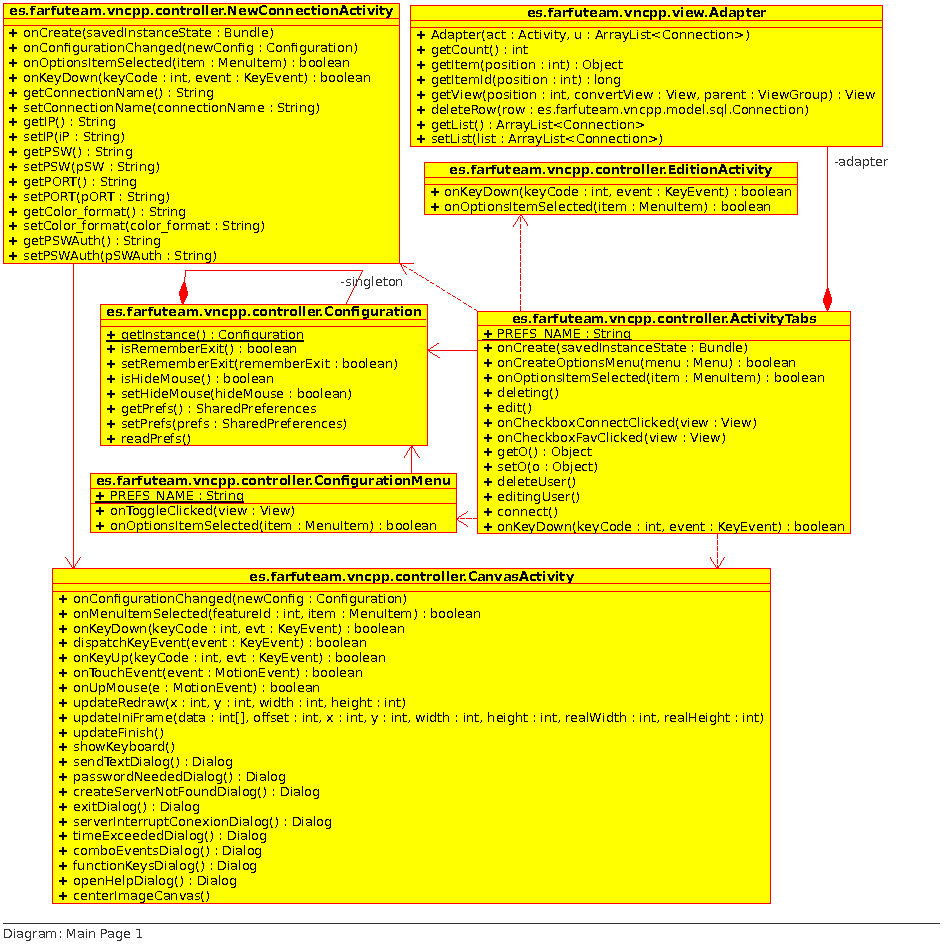
\includegraphics[scale=1]{Main.pdf}
\end{center}
\caption{Diagrama principal}
\end{figure}

Adapter es una clase configurar cada elemento de la lista de conexiones y la lista de favoritos. Las dos clases encargadas de la construcción estas listas son ListFragmentTab y ListFragmentTabFav, ambas se apollan en la clase Adapter para construirse.\\

CanvasActivity\\

\subsection{Parte escrita en C/C++}


